\documentclass[aspectratio=169,10pt]{beamer}

\usetheme[progressbar=frametitle]{metropolis}
\definecolor{kirmizi}{HTML}{A32638}
\definecolor{sari}{HTML}{FDB912}
\definecolor{mor}{HTML}{B6548F}
\setbeamercolor{frametitle}{bg=kirmizi, fg=sari}
\setbeamercolor{progress bar}{fg=sari, bg=kirmizi!30}
\setbeamercolor{title separator}{fg=kirmizi}
\setbeamercolor{progress bar in head/foot}{fg=sari, bg=kirmizi!30}
\setbeamercolor{progress bar in section page}{fg=sari, bg=kirmizi!30}
\setbeamercolor{alerted text}{fg=mor!140}
\setbeamercolor{palette primary}{bg=kirmizi, fg=sari}
\setbeamercolor{block title example}{fg=mor!140}

\usepackage[utf8]{inputenc}
\usepackage[T1]{fontenc}
\usepackage{amsmath,amssymb,amsthm,mathtools}
\usepackage{tikz}
\usetikzlibrary{positioning,arrows.meta,calc,fit,shapes.geometric}
\usepackage{booktabs}
\usepackage[style=authoryear, backend=biber, maxcitenames=2, uniquelist=false]{biblatex}
\addbibresource{../Library.bib}
\renewcommand*{\bibfont}{\scriptsize}

\newcommand{\toolname}{Coppula}
\newcommand{\Secure}{\textsf{Secure}}
\newcommand{\Insecure}{\textsf{Insecure}}
\newcommand{\F}{\mathbb{F}_2}
\newcommand{\Ws}{\mathcal{W}}
\newcommand{\Rs}{\mathcal{R}}
\newcommand{\Ss}{\mathcal{S}}
\newcommand{\law}[1]{\mathcal{L}_{#1}}
\newcommand{\va}{\mathbf{a}}
\newcommand{\vb}{\mathbf{b}}
\newcommand{\vw}{\mathbf{w}}
\newcommand{\CeqP}{\mathrm{C}_{=}\mathrm{P}}
\newcommand{\sharpP}{\#\mathrm{P}}

\definecolor{hlprobe}{RGB}{235,129,27}   % probed wires
\definecolor{hlsafe}{RGB}{35,138,94}     % safe / secure
\definecolor{hlbad}{RGB}{200,50,50}      % leaking
\definecolor{hlrand}{RGB}{60,110,200}    % randomness

\title{Verification of Probing Security for Masked Circuits}
\subtitle{A Constructive Approach and Theoretical Study}
\author{Kağan Gülsüm}
\institute{Sabancı University --- M.Sc. Thesis Defense\\{\scriptsize Supervisor: \textit{Asst. Prof. Süha Orhun Mutluergil}}}
\date{July 21, 2026}

% =====================================================================
% Running example: 2-share DOM-AND.
% =====================================================================
\tikzset{
  wire/.style={draw, rounded corners=2pt, minimum height=5.5mm, minimum width=11mm,
               inner sep=2pt, font=\small, fill=white},
  inwire/.style={wire, fill=black!5},
  randw/.style={wire, draw=hlrand, thick, fill=hlrand!10},
  probed/.style={draw=hlprobe, very thick, fill=hlprobe!15},
  safe/.style={draw=hlsafe, very thick, fill=hlsafe!12},
  leaky/.style={draw=hlbad, very thick, fill=hlbad!12},
  cwire/.style={-{Stealth[length=1.6mm]}, black!60},
  gsym/.style={circle, draw=black!60, fill=white, inner sep=0.3pt, font=\tiny},
}
\newcommand{\domand}[1]{%
\scalebox{0.88}{\begin{tikzpicture}[node distance=3.5mm and 9mm, #1]
  % products (middle column)
  \node[wire, wu0/.try]  (u0)  {$u_0$};
  \node[wire, below=of u0, wp01/.try] (p01) {$p_{01}$};
  \node[wire, below=13mm of p01, wp10/.try] (p10) {$p_{10}$};
  \node[wire, below=of p10, wu1/.try]  (u1)  {$u_1$};
  % inputs (left column)
  \node[inwire, left=9mm of u0, yshift=-2mm, wa0/.try] (a0) {$x_0$};
  \node[inwire, below=of a0] (a1) {$x_1$};
  \node[inwire, below=of a1, wb0/.try] (b0) {$y_0$};
  \node[inwire, below=of b0] (b1) {$y_1$};
  % masked cross terms, the shared fresh mask sits between them
  \node[wire, right=of p01, wc01/.try] (c01) {$c_{01}$};
  \node[wire, right=of p10, wc10/.try] (c10) {$c_{10}$};
  \node[randw, wr/.try] (r) at ($(c01)!0.5!(c10)$) {$r$};
  % outputs
  \node[wire, right=10mm of c01, yshift=4mm, ws0/.try] (s0) {$s_0$};
  \node[wire, right=10mm of c10, yshift=-4mm, ws1/.try] (s1) {$s_1$};
  % edges, each into the mid-point of the target's near side
  \draw[cwire] (a0.east) -- (u0.west);   \draw[cwire] (b0.east) -- (u0.west);
  \draw[cwire] (a0.east) -- (p01.west);  \draw[cwire] (b1.east) -- (p01.west);
  \draw[cwire] (a1.east) -- (p10.west);  \draw[cwire] (b0.east) -- (p10.west);
  \draw[cwire] (a1.east) -- (u1.west);   \draw[cwire] (b1.east) -- (u1.west);
  \draw[cwire] (p01.east) -- (c01.west); \draw[cwire] (r.north) -- (c01.south);
  \draw[cwire] (p10.east) -- (c10.west); \draw[cwire] (r.south) -- (c10.north);
  \draw[cwire] (u0.east) -- (s0.west);   \draw[cwire] (c01.east) -- (s0.west);
  \draw[cwire] (u1.east) -- (s1.west);   \draw[cwire] (c10.east) -- (s1.west);
  % gate types
  \node[gsym] at (u0.north west)  {$\odot$};
  \node[gsym] at (p01.north west) {$\odot$};
  \node[gsym] at (p10.north west) {$\odot$};
  \node[gsym] at (u1.north west)  {$\odot$};
  \node[gsym] at (c01.north west) {$\oplus$};
  \node[gsym] at (c10.north west) {$\oplus$};
  \node[gsym] at (s0.north west)  {$\oplus$};
  \node[gsym] at (s1.north west)  {$\oplus$};
\end{tikzpicture}}}

\begin{document}
\maketitle

% ---------------------------------------------------------------------
\begin{frame}{The story}
  \begin{enumerate}
    \item<1-> Masked circuits defend against side-channel attacks, but masking is
      easy to get subtly wrong. So, we want to \emph{verify} it, exactly.
    \item<2-> Deciding even one observation is provably hard
      ($\CeqP$-complete), so we cannot count to find an answer.
    \item<3-> Instead, we certify security \emph{constructively}, giving a proof of
      independence via a \emph{coupling} of the circuit's randomness.
    \item<4-> We present \toolname, a Lean~4 verifier built on this idea, with three
      components: a rewrite engine, a subset-space traversal, and a
      probe-set extension.
    \item<5-> It verifies a suite of masked gadgets exactly, and the coupling
      view proves to be helpful.
  \end{enumerate}
\end{frame}

% =====================================================================
\section{Motivation \& Model}
% =====================================================================

\begin{frame}{Side-channel attacks}
  A cipher can be secure on paper and insecure on the bench.
  \begin{itemize}
    \item A real device leaks through power draw, timing, electromagnetic
      emanation; all of which vary with the \emph{data} it handles.
    \item Differential power analysis \parencite{kocher1999differential} correlates many power
      traces against a guess of an intermediate value, and may recover the key.
  \end{itemize}
  \medskip
  \begin{alertblock}{}
    So, the insecurity lies not in the mathematics behind the cipher, but in the way
    the hardware computes it.
  \end{alertblock}
\end{frame}

\begin{frame}{Masking --- and our running example}
  \emph{Boolean masking} \parencite{chari1999towards} splits each secret into shares,
  $x = x_0 \oplus x_1$, with $x_0$ uniformly random, and computation happens on
  shares, never directly on secrets. Then, the cost of attacking grows exponentially in the number
  of shares.
  \medskip
  \begin{columns}[c]
    \begin{column}{0.52\textwidth}
      \centering
      \domand{}
    \end{column}
    \begin{column}{0.44\textwidth}
      \textbf{DOM-AND} \parencite{gross2016domain}: a masked AND gate, with two shares per input,
      and a fresh mask $r$.
      \medskip
      \begin{itemize}
        \item computes a sharing $s_0 \oplus s_1 = x \odot y$,
        \item the cross terms $p_{01}, p_{10}$ mix shares of \emph{both}
          secrets --- the delicate part,
        \item $r$ re-masks them before they meet an output.
      \end{itemize}
      \medskip
      This gadget accompanies us for the rest of the talk.
    \end{column}
  \end{columns}
\end{frame}

\begin{frame}{The probing model}
  Reasoning about noisy traces directly is unwieldy. Luckily we have an
  abstraction \parencite{10.1007/978-3-540-45146-4_27}:
  \begin{block}{$d$-probing security}
    An adversary picks any $d$ wires and is handed their \emph{exact} values.
    The circuit is $d$-probing secure when no such choice distinguishes one
    secret assignment from another.
  \end{block}
  \medskip
  \begin{columns}[c]
    \begin{column}{0.5\textwidth}
      \centering
      \domand{wc01/.style={wire,probed}}
    \end{column}
    \begin{column}{0.46\textwidth}
      \begin{itemize}
        \item<2-> Now, security becomes a \emph{combinatorial} property of the
          circuit, algortihmically decidable in principle.
        \item<3-> And thankfully, the abstraction is faithful: probing security implies
          noisy-leakage security \parencite{duc2014unifying}. We take
          $d$-probing security as the target and do not revisit this bridge.
      \end{itemize}
    \end{column}
  \end{columns}
\end{frame}

\begin{frame}{The problem}
  \textbf{Setting.} We work with arithmetic circuits over $\F$, two-input $\oplus$ and
  $\odot$ gates, where inputs are partitioned into secrets $\Ss$, randoms $\Rs$, publics
  $\mathcal{P}$. We have value-based leakage, so, no glitches, and also no composition.
  \medskip
  \begin{block}{Exact verification of $d$-probing security}
    One should decide, for \emph{every} one of the $\sum_{i \le d} \binom{|\Ws|}{i}$
    observation sets, whether it is independent of the secrets.
    \begin{itemize}
      \item $\Secure$ \;\;\; $\Rightarrow$ every observation set accounted for,
      \item $\Insecure$ \; $\Rightarrow$ a specific leaking observation as
        witness.
    \end{itemize}
  \end{block}
  \medskip
  \begin{itemize}
    \item<2-> Two difficulties arise: a \emph{single} probe already asks a question
      about a distribution over all of $\{0,1\}^{\Rs}$,
    \item<3-> and there are combinatorially many probes to settle.
  \end{itemize}
\end{frame}

% =====================================================================
\section{How Hard Is One Probe?}
% =====================================================================

\begin{frame}{Warm-up: three views of secret-independence}
  Fix a probe $O$ (a tuple $\mathbf{w}$ of wires). Write $\law{\va}(O)$ for its
  distribution over a uniform tape $\rho \in \{0,1\}^{\Rs}$, and
  $N_{\va}(o) = |\{\rho : O(\rho;\va) = o\}|$ for the tape counts.
  \medskip
  \begin{enumerate}
    \item<1-> \textbf{Distributional.} \; $\law{\va}(O) = \law{\vb}(O)$ for all
      secrets $\va, \vb$. \hfill {\small \emph{(the definition)}}
    \item<2-> \textbf{Counting.} \; $N_{\va}(o) = N_{\vb}(o)$ for every
      observation $o$, i.e. two histograms of integers coincide.
      
      {\small \emph{$\to$ this section}}
    \item<3-> \textbf{Coupling.} \; there exists a bijection
      $\varphi$ of the tapes such that $O(\rho;\va) = O(\varphi(\rho);\vb)$.
      
      {\small \emph{$\to$ next section}}
  \end{enumerate}
  \medskip
  \onslide<4->{
  All three are equivalent --- but they are \emph{not} equally usable.
  The counting view tells us what a verification procedure should not attempt
  directly; the coupling view tells us what it might be able to acomplish.}
\end{frame}

\begin{frame}{Counting is intractable}
  \begin{block}{Theorem (thesis, Ch.~4)}
    Computing one tape count $N_{\va}(o)$ is $\sharpP$-complete
    \parencite{valiant1979complexity}. And deciding $\law{\va}(O) = \law{\vb}(O)$ is
    $\CeqP$-complete \parencite{wagner1986complexity}.
  \end{block}
  \medskip
  \emph{Hardness, briefly:} for formulas $\varphi_0, \varphi_1$ over
  randoms $x_1, \dots, x_m$ and a single secret bit $s$, the wire
  \[
    w \;=\; \varphi_0 \,\oplus\, \bigl(s \odot (\varphi_0 \oplus \varphi_1)\bigr)
  \]
  reads $\varphi_0$ when $s=0$ and $\varphi_1$ when $s=1$. Then, the one-bit probe
  $\{w\}$ is secret-independent \emph{iff} $\#\varphi_0 = \#\varphi_1$. That is
  exactly the canonical $\CeqP$-complete question: \textsc{ExactSat}.
  \medskip

  \onslide<2->{One secret bit and one probed wire already suffice for the problem
  to be intractable; no feature of masking is what makes the problem hard.}
\end{frame}

\begin{frame}{What the placement tells}
  \begin{itemize}
    \item<1-> Observe that $\CeqP \subseteq \mathrm{P}^{\sharpP}$, so the decision never costs
      more than the counting. Another observation is the following: a formula is unsatisfiable
      exactly when its count is zero, i.e. $\mathrm{coNP} \subseteq \CeqP$. Hence, no
      polynomial exact decision exists unless $\mathrm{P} = \mathrm{NP}$.
    \item<2-> Both classes sit \emph{above the polynomial hierarchy} (due to Toda).
      A single probe is already there, and full verification universally
      quantifies over exponentially many such instances.
  \end{itemize}
  \medskip
  \begin{exampleblock}{Consequence}
    We do not compute or compare the counts. We certify security
    \emph{constructively}: by exhibiting, for each probe, a measure-preserving
    relabelling of the randomness under which the secrets visibly cancel.
    A witness proves independence without explicitly counting --- at the price of
    completeness!
  \end{exampleblock}
\end{frame}

% =====================================================================
\section{Security Is a Coupling}
% =====================================================================

\begin{frame}{One substitution, on the running example}
  \small
  Probe the masked cross term: $c_{01} = x_0 \odot y_1 \oplus r$.
  \medskip
  \begin{columns}[c]
    \begin{column}{0.5\textwidth}
      \centering
      \domand{wc01/.style={wire,probed}, wr/.style={wire,randw,safe}}
    \end{column}
    \begin{column}{0.46\textwidth}
      Apply the substitution
      $\sigma = \bigl(r \mapsto x_0 \odot y_1 \oplus r\bigr)$:
      \[
        c_{01}\,\sigma
        \;=\; x_0 \odot y_1 \oplus (x_0 \odot y_1 \oplus r)
        \;=\; r .
      \]
      \begin{itemize}
        \item<2-> The probe is now \emph{syntactically secret-free}: it is
          uniform, whatever the secrets are.
        \item<3-> And $\sigma$ is not just a change of variables. It induces a
          \emph{bijection} $\widehat{\sigma}$ of the tape space
          $\{0,1\}^{\Rs}$ by translating one coordinate --- a \emph{shear}.
      \end{itemize}
    \end{column}
  \end{columns}
  \medskip
  \onslide<4->{Key identity: \; $(\mathbf{w}\sigma)(\rho) = \mathbf{w}(\widehat{\sigma}(\rho))$
  --- the syntactic step and the semantic relabelling agree.}
\end{frame}

\begin{frame}{Couplings}
  The classical idea (\parencite{barthe2017coupling} for probabilistic programs) to prove that two
  distributions are equal without explicitly computing them is by \emph{linking their
  sources}. Our two laws are pushforwards of the \emph{same} uniform tape. So we should
  cleverly link those tapes.
  \medskip
  \begin{block}{Definition (coupling function)}
    A \emph{coupling function} from $\va$ to $\vb$ for a probe $O$ is a
    bijection $\varphi : \{0,1\}^{\Rs} \to \{0,1\}^{\Rs}$ with
    \[
      O(\rho;\va) \;=\; O\bigl(\varphi(\rho);\vb\bigr)
      \qquad \text{for every tape } \rho .
    \]
  \end{block}
  \begin{itemize}
    \item<2-> A bijection of a finite set preserves the uniform law
      trivially. The identity says that a run under $\va$ is
      reproduced, observation for observation, under $\vb$. This is a
      \emph{diagonal} coupling of the two laws. It proves that the
      distributions on the observation set are the same for those two
      secrets.
    % \item<3-> The family $\Phi = \{\Phi_{\va,\vb}\}$ over ordered secret pairs
    %   forms a \emph{groupoid}: $\Phi_{\va,\va} = \mathrm{id}$,
    %   $\Phi_{\vb,\va} = \Phi_{\va,\vb}^{-1}$,
    %   $\Phi_{\vb,\mathbf{c}} \circ \Phi_{\va,\vb} = \Phi_{\va,\mathbf{c}}$.
    %   One anchor row generates the rest.
  \end{itemize}
\end{frame}

\begin{frame}{Security \emph{is} a coupling}
  \small
  \begin{block}{Theorem}
    A probe $O$ is secret-independent \emph{iff} for every ordered pair
    $\va, \vb$ there is a coupling function from $\va$ to $\vb$ for $O$.
  \end{block}
  \medskip
  \emph{Proof sketch.}
  \begin{itemize}
    \item<2-> ($\Leftarrow$) Reindex by $\rho' = \varphi(\rho)$:
      \[
        N_{\va}(o) = \bigl|\{\rho : O(\rho;\va) = o\}\bigr|
        = \bigl|\{\rho : O(\varphi(\rho);\vb) = o\}\bigr|
        = N_{\vb}(o).
      \]
    \item<3-> ($\Rightarrow$) Sort the tapes by outcome:
      $F_{\va}(o) = \{\rho : O(\rho;\va) = o\}$. As $o$ varies these
      \emph{fibres} partition $\{0,1\}^{\Rs}$, and equal laws mean matching
      fibres have equal size, $|F_{\va}(o)| = |F_{\vb}(o)|$. So pick, for each
      $o$, any bijection $F_{\va}(o) \to F_{\vb}(o)$; their union is a
      bijection $\varphi$ of the whole tape space, and it sends every $\rho$
      to a tape with the \emph{same} observation, giving us a coupling function. \qed
  \end{itemize}
  \medskip
  \onslide<4->{
  \begin{alertblock}{This is an existence statement and not a procedure}
    The ($\Rightarrow$) direction matches fibres \emph{block by block}, and
    for that it needs the counts $N_{\va}(o)$, which are
    $\sharpP$-hard to compute. So, the theorem guarantees a coupling, it does not find one.
  \end{alertblock}}
\end{frame}

\begin{frame}{From substitutions to couplings --- the constructive route}
  \begin{itemize}
    \item<1-> Each substitution induces a shear, a bijection of the tapes.
      A \emph{sequence} of substitutions composes to a bijection
      $\varphi_{\va}$ --- one per secret assignment, since the contexts
      $e_i$ may mention secrets.
    \item<2-> If the sequence drives the probe to a secret-free form
      $\overline{O}$, then \emph{both} runs agree like the following:
      \[
        O\bigl(\varphi_{\va}(\rho);\va\bigr) \;=\; \overline{O}(\rho)
        \;=\; O\bigl(\varphi_{\vb}(\rho);\vb\bigr) .
      \]
    \item<3-> Chain through the common form as $\varphi_{\vb} \circ
      \varphi_{\va}^{-1}$, and one gets a coupling function from $\va$ to $\vb$ --- for
      \emph{every} pair of secrets at once, from one derivation.
    \item<4-> So a successful rewrite derivation is not a simple $\Secure$ verdict.
      It is an explicit, checkable, reusable \emph{certificate}.
  \end{itemize}
  \medskip
  \onslide<4->{
  \begin{exampleblock}{}
    This is the design principle of \toolname: replace intractable counting by
    the search for a coupling, building it one substitution at a time.
  \end{exampleblock}}
\end{frame}

% =====================================================================
\section{\toolname: Three Components}
% =====================================================================

\begin{frame}{Pipeline overview}
  \centering
  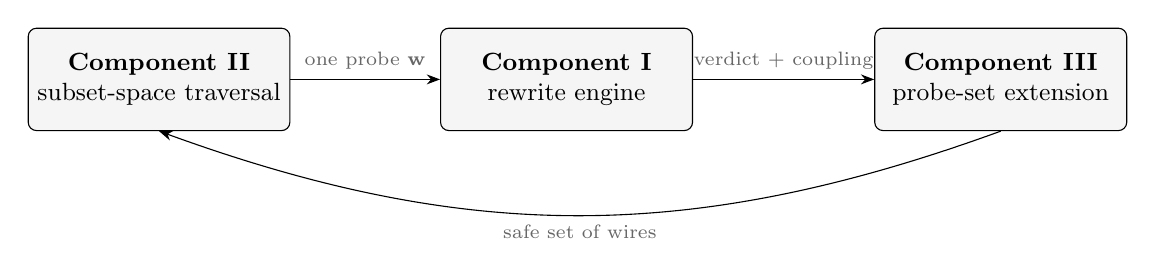
\begin{tikzpicture}[node distance=6mm and 10mm,
      comp/.style={draw, rounded corners=3pt, align=center, minimum height=13mm,
                   minimum width=32mm, font=\small, fill=black!4},
      lbl/.style={font=\scriptsize, text=black!60}]
    \node[comp] (c2) {\textbf{Component II}\\ subset-space traversal};
    \node[comp, right=19mm of c2] (c1) {\textbf{Component I}\\ rewrite engine};
    \node[comp, right=23mm of c1] (c3) {\textbf{Component III}\\ probe-set extension};
    \draw[-{Stealth}] (c2) -- node[lbl, above]{one probe $\vw$} (c1);
    \draw[-{Stealth}] (c1) -- node[lbl, above]{verdict $+$ coupling} (c3);
    \draw[-{Stealth}] (c3.south) to[bend left=20]
      node[lbl, below]{safe set of wires} (c2.south);
  \end{tikzpicture}
  \medskip
  \begin{itemize}
    \item<2-> \textbf{I} decides a \emph{single} probe, by construction.
    \item<3-> \textbf{II} sweeps \emph{every} $d$-subset without explicitly enumerating
      them.
    \item<4-> \textbf{III} amplifies one certificate into a whole \emph{safe
      set}, shrinking the space \textbf{II} must sweep.
  \end{itemize}
\end{frame}

\begin{frame}{Component I: the rewrite engine}
  Decides one probe $\mathbf{w}$ by substituting randoms away, one at a time, driving the
  observation toward a secret-free form.
  \medskip
  \begin{itemize}
    \item<1-> \textbf{Tiered.} A cheap single-occurrence rule first ($r$ occurs
      once across $\mathbf{w}$: substitute, done); with a complete substitution loop
      behind it.
    \item<2-> \textbf{Sound.} Every step is a shear, so any $\Secure$ verdict
      carries a genuine coupling (Theorem, Ch.~5).
    \item<3-> \textbf{Incomplete, knowingly.} A probe can be independent for
      reasons no relabelling of this kind captures --- this is the price of the
      hardness result.
  \end{itemize}
  \medskip
  \onslide<4->{
  On the example: $c_{01} \xrightarrow{\;\;r \;\mapsto\; a_0 \odot b_1 \oplus r\;\;} r$
  is a single step discharge, which is $\Secure$, and records a coupling.}
\end{frame}

\begin{frame}{Component I: why factoring}
  Some masks are buried inside \emph{products}, where substitution cannot
  reach them.
  \medskip
  \begin{itemize}
    \item<1-> Substituting $r \mapsto e \oplus r$ needs $r$ to occur as a
      \emph{summand}; in $u \odot r \oplus u \odot v$ every occurrence of $r$
      is trapped inside a product.
    \item<2-> \textbf{Multiplicative factoring} pulls the common factor out,
      \[
        u \odot r \,\oplus\, u \odot v \;\longmapsto\; u \odot (r \oplus v) ,
      \]
      and the hidden random surfaces as a summand again, ready to substitute.
    \item<3-> Factoring is applied lazily, on demand, between substitution
      attempts; the engine interleaves the two until the probe is discharged
      or no rule applies.
  \end{itemize}
  % \medskip
  % \onslide<4->{\emph{Caveat, stated openly:} factoring itself is not a shear
  % --- it changes the syntax, not the tapes. This has a consequence for how we
  % extend probes, coming up in Component III.}
\end{frame}

\begin{frame}{Component II: covering all probes}
  Certifying each $d$-subset in turn is infeasible. Instead the space lives as
  a \emph{worklist} of factors $\langle (c_1, W_1), \dots, (c_m, W_m) \rangle$,
  ``draw $c_j$ wires from each $W_j$'', and we split recursively, in the manner of
  maskVerif \parencite{10.1007/978-3-030-29959-0_15}:
  \medskip
  \begin{itemize}
    \item<1-> Initially, try to discharge a whole batch at once: if the \emph{union} of
      its wires is jointly secret-free, every probe inside is also settled ---
      prune the branch.
    \item<2-> On failure, certify one representative \emph{probe} $\mathbf{w}$ (one
      probe of the target size, $c_j$ wires from each factor), grow it into a
      safe set (Component III), and split every factor along
      safe~/~unsafe regions. Recurse on the resulting cells; the all-safe cell needs
      no visit.
  \end{itemize}
  \medskip
  \begin{block}{Theorem (exhaustiveness, Ch.~5)}
    The recursion visits every $d$-subset exactly once. The proof reads
    Vandermonde's identity
    $\binom{m+n}{d} = \sum_k \binom{m}{k}\binom{n}{d-k}$
    at the level of \emph{sets}: the cells genuinely partition the probes,
    they do not merely count them.
  \end{block}
  \medskip
  \onslide<3->{The delicate point is that the split must \emph{lose nothing},
  and we proved that it does not.}
\end{frame}

\begin{frame}{Component III: growing safe sets}
  A discharged probe is a coupling --- but can the \emph{same} coupling cover more
  wires?
  \medskip
  \begin{columns}[c]
    \begin{column}{0.5\textwidth}
      \centering
      \domand{wc01/.style={wire,safe}, wu0/.style={wire,safe},
              wu1/.style={wire,safe}, wp01/.style={wire,safe}}
    \end{column}
    \begin{column}{0.46\textwidth}
      \begin{itemize}
        \item<1-> A wire $u$ joins the safe set of coupling $\varphi$ when the
          composite $u \circ \varphi$ is secret-free.
        \item<2-> Exact test: a function depends on a variable iff the
          variable occurs in its \emph{ANF} --- so the endpoint test is
          to send expressions into their normal froms.
        \item<3-> One certificate, with more wires: the whole safe set is settled
          by a single discharge, and Component II skips it.
      \end{itemize}
    \end{column}
  \end{columns}
\end{frame}

\begin{frame}{Component III: three mechanisms}
  \begin{itemize}
    \item<1-> \textbf{Closure} --- build-time, entropy-style deduction
      ($H(u \mid \vw) = 0$). Works locally, but the candidate pool deep in the
      recursion is scattered. A cheap step but weak.
    \item<2-> \textbf{Replay} --- re-run the derivation on the candidate wire
      \parencite{barthe2015verified}. An imperfect fit for us because we \emph{factor},
      and factoring is not a replayable step.
    \item<3-> \textbf{Coupling} --- apply the recorded tape bijection and test
      the ANF endpoint. Exact, and independent of how the derivation was
      found.
  \end{itemize}
  \medskip
  \begin{block}{Proposition (nesting, Ch.~5)}
    $\text{closure} \subseteq \text{replay} \subseteq \text{coupling}$ ---
    every wire the cheaper mechanisms admit, the coupling admits too.
    \toolname{} adopts the coupling approach.
  \end{block}
\end{frame}

\begin{frame}{Component III: the test}
  \small
  Take the certified probe $\mathbf{w}$ with coupling $\varphi$, and a candidate wire $u$ from the current pool.
  Decide whether $u \circ \varphi$ secret-free?
  \begin{block}<1->{Phase 1 --- fast reject (probabilistic, may only \emph{reject})}
    Sample tapes; evaluate $u \circ \varphi$ twice per tape, secrets drawn at
    random vs.\ all zero. A disagreement proves $u \circ \varphi$ moves with
    the secrets: drop $u$. Agreement proves nothing, survivors move on.
  \end{block}
  \begin{block}<2->{Phases 2--3 --- exact ($\F$ cancellation, then ANF)}
    A function depends on a variable iff the variable occurs in its unique
    multilinear normal form. So admit $u$ exactly when no secret survives in
    the ANF of $u \circ \varphi$ (Lemma, Ch.~5).
  \end{block}
  \medskip
  \onslide<3->{\textbf{Why blinded wires are safe to add.} For an admitted $u$,
  $u(\varphi_{\va}(\rho); \va) = \overline{u}(\rho)$, a function of $\rho$
  alone. Since $\varphi_{\va}$ preserves the uniform law, the \emph{joint} law
  of all admitted wires under $\va$ is that of
  $(\overline{u}(\rho))_{u}$, which mentions no secret (Theorem, Ch.~5).}
\end{frame}

% \begin{frame}{The running example: order two}
%   \small
%   What about probing \emph{both} masked cross terms?
%   \medskip
%   \begin{columns}[c]
%     \begin{column}{0.5\textwidth}
%       \centering
%       \domand{wc01/.style={wire,leaky}, wc10/.style={wire,leaky},
%               wr/.style={wire,randw}}
%     \end{column}
%     \begin{column}{0.46\textwidth}
%       \begin{itemize}
%         \item<1-> Individually, $c_{01}$ and $c_{10}$ are uniform --- $r$ masks
%           each.
%         \item<2-> Jointly, the \emph{shared} mask cancels:
%           \[
%             c_{01} \oplus c_{10} = a_0 \odot b \,\oplus\, a \odot b_0 ,
%           \]
%           a secret-dependent value. No substitution can save it; the engine
%           returns $\Insecure$ with this pair as witness.
%         \item<3-> So DOM-AND is secure at order one, insecure at order two ---
%           exactly as designed, and exactly what \toolname{} reports.
%       \end{itemize}
%     \end{column}
%   \end{columns}
% \end{frame}

% =====================================================================
\section{Implementation \& Evaluation}
% =====================================================================

\begin{frame}{Implementation details}
  \toolname{} is implemented in \textbf{Lean 4}.
  \medskip
  \begin{itemize}
    \item<1-> \textbf{Hash-consed DAG} expression representation with
      canonicalization --- structural sharing makes equality checks and
      substitution efficient time- and memory-wise.
    \item<2-> \textbf{Multiplicative factoring} as a normal-form pass over the
      DAG, applied lazily.
    \item<3-> \textbf{Bit-sliced ANF endpoint test} for the extension:
      word-parallel evaluation decides secret-freeness of $u \circ \varphi$
      exactly.
  \end{itemize}
  \medskip
  \onslide<4->{Design and proofs are implementation-agnostic; these choices
  simply make algorithms fast.}
\end{frame}

  \begin{frame}{Evaluation: outcomes}
  \small
  Forty configurations at orders 1--4: ISW multiplications, DOM and TI ANDs,
  refresh gadgets, Keccak $\chi$ (DOM and TI sharings), and the TI S-boxes and
  quadratic sharings of Bilgin et al. Every verdict matches the ground truth,
  and every $\Insecure$ comes with a concrete witness observation.
  \medskip
  \begin{itemize}
    \item<1-> \textbf{DOM-AND} (2 shares): $\Secure$ at order 1, the witness
      pair $\{c_{01}, c_{10}\}$ at order 2 --- our running example.
    \item<2-> \textbf{Four-share $x \oplus yz$ TI} \parencite{bilgin2015threshold}:
      certified secure at orders 1 and 2, insecure at order 3 --- the
      \emph{expected} behaviour of a first-order threshold implementation.
    \item<3-> \textbf{The factoring family} ($d{+}1$ quadratic S-boxes,
      $Q^3\!/Q^4$): randomness-free sharings whose certification must factor
      first. A factoring-free, maskVerif-style replay engine false-reports
      $\Insecure$ on five of them; \toolname{} verifies every one --- and the
      two it does report insecure are exactly the quadratic classes with no
      uniform three-share TI.
  \end{itemize}
  \medskip
  \onslide<4->{(Full extension-comparison table @ the appendix slides.)}
\end{frame}

\begin{frame}{Evaluation: is the extension worth it?}
  \small
  \begin{columns}[c]
    \begin{column}{0.5\textwidth}
      \centering
      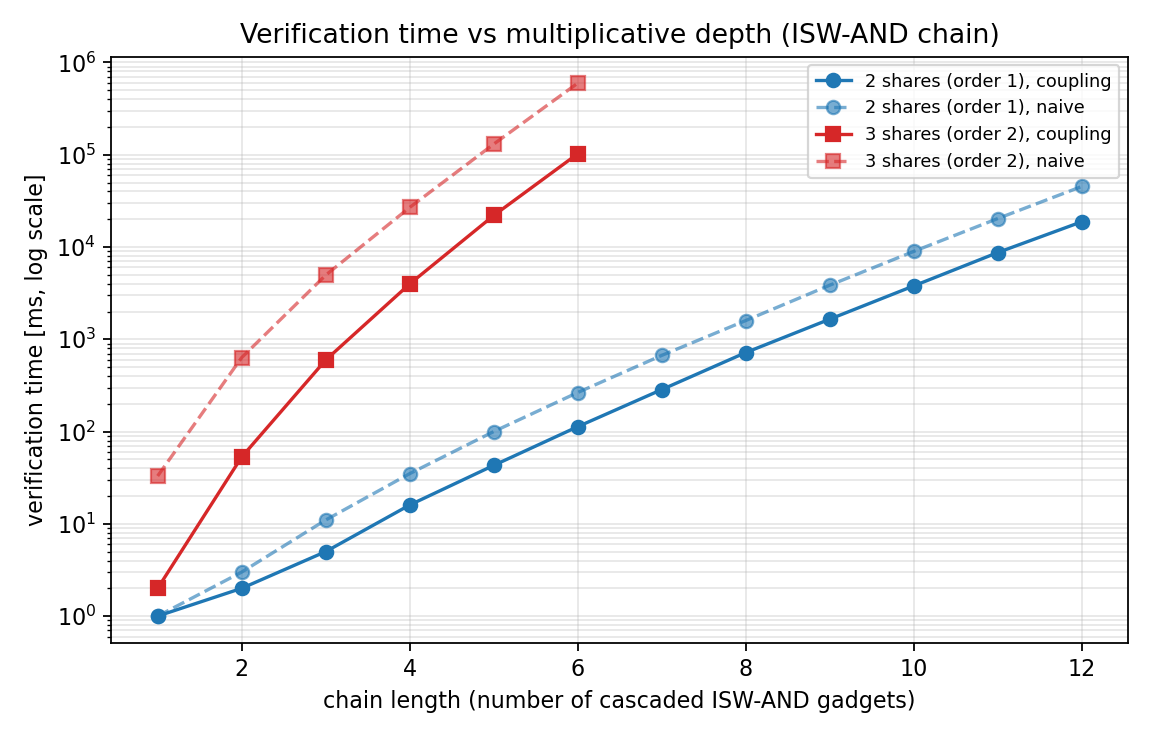
\includegraphics[width=1.05\textwidth]{../Figures/scaling.png}\\
      {\scriptsize Verification time versus circuit depth.}
    \end{column}
    \begin{column}{0.46\textwidth}
      \begin{itemize}
        \item<1-> Coupling matches replay's yield \emph{to the digit} wherever
          replay is right (five-share ISW: $4735$ discharges, $8078$ free
          wires on both) --- and keeps the correct verdict on the five rows
          where replay false-reports $\Insecure$.
        \item<2-> Closures keep the verdicts but lose the yield: $14$ vs.\
          $537$ free wires on Fides, $632{,}834$ vs.\ $4735$ discharges on
          five-share ISW --- the split degrades toward enumeration.
        \item<3-> The extension pays for itself: Fides certifies $537$ wires
          from $55$ discharges; five-share ISW falls from ${\sim}609$\,s
          (no extension) to under $2$\,s.
      \end{itemize}
    \end{column}
  \end{columns}
\end{frame}

% =====================================================================
\section{Wrap-up}
% =====================================================================

\begin{frame}{Limitations and future work}
  \begin{itemize}
    \item<1-> \textbf{Model.} Our model is value-based leakage only: glitches and
      transitions are out of scope; so is composition. So we show single-circuit, exact
      probing security.
    \item<2-> \textbf{Larger fields.} The core --- shears, couplings, ANF ---
      is already field-agnostic; lifting the implementation beyond $\F$ is
      engineering plus a normal-form choice. (Also, the power of Schwartz--Zippel
      can come into picture here.)
    \item<3-> \textbf{Composing couplings.} for unions of safe sets using
      couplings as a guide.
    \item<4-> \textbf{More.} smarter factoring heuristics; exploiting circuit
      symmetries to quotient the subset space.
  \end{itemize}
\end{frame}

\begin{frame}{Contributions}
  \begin{enumerate}
    \item<1-> \textbf{Placement.} We show that: counting is
      $\sharpP$-complete, deciding is $\CeqP$-complete --- above the
      polynomial hierarchy, ruling out the counting route.
    \item<2-> \textbf{A rigorous coupling account of probing security.}
      Security \emph{is} the existence of a family of coupling functions, the
      family is a groupoid, and substitutions construct it.
    \item<3-> \textbf{\toolname.} Made up of a sound rewrite engine (with factoring), an
      exhaustive subset-space traversal,
      and a probe-set extension with a proven mechanism hierarchy
      $\text{closure} \subseteq \text{replay} \subseteq \text{coupling}$.
    \item<4-> \textbf{Evaluation.} We present exact verdicts, with witnesses, across a
      suite of masked gadgets, and the coupling extension wins in coverage.
  \end{enumerate}
\end{frame}

\begin{frame}[standout]
  Thank you!\\[2ex]
  {\normalsize Questions?}
\end{frame}

% =====================================================================
\appendix
\section*{Backup}
% =====================================================================

\begin{frame}{Backup: extension comparison (I/IV)}
  \scriptsize
  Each entry: Coupling\,/\,Replay\,/\,Closure. Verdict S $=$ \Secure{},
  I $=$ \Insecure{}; $\dagger$ marks replay's false-$\Insecure$s.
  \medskip

  \setlength{\tabcolsep}{5pt}
  \begin{tabular}{@{}l c c c c c@{}}
  \toprule
  Circuit & $d$ & Verdict & Time [ms] & Discharges & Free wires \\
  \midrule
  \multicolumn{6}{@{}l}{\textbf{ISW multiplication}}\\
  \quad $2$ sh.        & $1$ & S/S/S & $0/0/1$              & $7/7/15$              & $2/2/0$          \\
  \quad $3$ sh.        & $2$ & S/S/S & $3/1/34$             & $34/34/309$           & $31/31/8$        \\
  \quad $4$ sh.        & $3$ & S/S/S & $46/37/3190$         & $338/338/10770$       & $437/437/439$    \\
  \quad $5$ sh.        & $4$ & S/S/S & $1125/845/409472$    & $4735/4735/632834$    & $8078/8078/37513$\\
  \addlinespace
  \multicolumn{6}{@{}l}{\textbf{DOM AND}}\\
  \quad $2$ sh.        & $1$ & S/S/S & $1/0/0$              & $11/11/15$            & $2/2/0$          \\
  \quad $2$ sh.        & $2$ & I/I/I & $0/0/1$              & $2/2/6$               & $0/0/2$          \\
  \quad $3$ sh.        & $2$ & S/S/S & $5/4/35$             & $88/88/325$           & $44/44/7$        \\
  \quad $4$ sh.        & $3$ & S/S/S & $104/90/3419$        & $859/859/13291$       & $784/784/532$    \\
  \bottomrule
  \end{tabular}
\end{frame}

\begin{frame}{Backup: extension comparison (II/IV)}
  \scriptsize
  \setlength{\tabcolsep}{5pt}
  \begin{tabular}{@{}l c c c c c@{}}
  \toprule
  Circuit & $d$ & Verdict & Time [ms] & Discharges & Free wires \\
  \midrule
  \multicolumn{6}{@{}l}{\textbf{Trichina AND}}\\
  \quad well-formed    & $1$ & S/S/S & $0/1/1$              & $11/11/15$            & $2/2/0$          \\
  \quad mis-associated & $1$ & I/I/I & $1/0/1$              & $10/10/12$            & $1/1/0$          \\
  \addlinespace
  \multicolumn{6}{@{}l}{\textbf{TI AND}}\\
  \quad $3$ sh.        & $1$ & S/S/S & $0/0/1$              & $9/9/27$              & $9/9/0$          \\
  \quad $3$ sh.        & $2$ & I/I/I & $1/1/1$              & $10/10/10$            & $5/5/2$          \\
  \addlinespace
  \multicolumn{6}{@{}l}{\textbf{Mask refreshing}}\\
  \quad additive, $3$ sh. & $2$ & S/S/S & $0/0/0$           & $6/6/8$               & $1/1/0$          \\
  \quad additive, $4$ sh. & $3$ & S/S/S & $1/0/1$           & $11/11/17$            & $6/6/0$          \\
  \quad ISW, $3$ sh.      & $2$ & S/S/S & $0/0/0$           & $6/6/10$              & $4/4/0$          \\
  \quad ISW, $4$ sh.      & $3$ & S/S/S & $0/1/2$           & $12/12/51$            & $24/24/0$        \\
  \addlinespace
  \multicolumn{6}{@{}l}{\textbf{Keccak $\chi$}}\\
  \quad DOM, $2$ sh.   & $1$ & S/S/S & $14/11/29$           & $49/49/107$           & $29/29/5$        \\
  \quad DOM, $3$ sh.   & $2$ & S/S/S & $2807/1797/11563$    & $2865/2865/14047$     & $2671/2671/645$  \\
  \quad TI, $3$ sh.    & $1$ & S/S/S & $21/14/103$          & $43/43/183$           & $68/68/5$        \\
  \quad TI, $3$ sh.    & $2$ & I/I/I & $21/14/72$           & $57/57/352$           & $92/92/27$       \\
  \bottomrule
  \end{tabular}
\end{frame}

\begin{frame}{Backup: extension comparison (III/IV)}
  \scriptsize
  \setlength{\tabcolsep}{5pt}
  \begin{tabular}{@{}l c c c c c@{}}
  \toprule
  Circuit & $d$ & Verdict & Time [ms] & Discharges & Free wires \\
  \midrule
  \multicolumn{6}{@{}l}{\textbf{TI S-boxes and quadratic sharings}}\\
  \quad $Q^4_{12}$ direct, $2$ sh. & $1$ & S/I$^\dagger$/S & $2/2/5$      & $27/26/47$   & $16/16/10$ \\
  \quad $Q^4_{12}$ TI, $3$ sh.     & $1$ & S/S/S           & $5/4/25$     & $25/25/83$   & $30/30/6$  \\
  \quad Fides AB1, $4$ sh.         & $1$ & S/S/S           & $1941/972/36461$ & $55/55/1127$ & $537/537/14$ \\
  \quad $x+yz$ direct, $3$ sh.     & $1$ & S/S/S           & $1/0/3$      & $7/7/29$     & $10/10/0$  \\
  \quad $x+yz$ w/ CT, $3$ sh.      & $1$ & S/S/S           & $1/1/3$      & $11/11/29$   & $9/9/0$    \\
  \quad $x+yz$, $4$ sh.            & $2$ & S/S/S           & $11/8/170$   & $78/78/767$  & $115/115/20$\\
  \quad $x+yz$, $4$ sh.            & $3$ & I/I/I           & $11/7/8$     & $102/102/72$ & $99/99/15$ \\
  \quad $x+yz+xyz$, $4$ sh.        & $1$ & S/S/S           & $45/18/175$  & $31/31/167$  & $63/63/1$  \\
  \quad $xy$ virtual var.          & $1$ & S/S/S           & $3/1/17$     & $9/9/55$     & $23/23/0$  \\
  \quad $xy$ virtual share         & $1$ & S/S/S           & $1/0/7$      & $9/9/37$     & $15/15/0$  \\
  \quad $xy$, $4{\to}3$ sh.        & $1$ & S/S/S           & $1/1/3$      & $11/11/25$   & $8/8/0$    \\
  \bottomrule
  \end{tabular}
\end{frame}

\begin{frame}{Backup: extension comparison (IV/IV)}
  \scriptsize
  \setlength{\tabcolsep}{5pt}
  \begin{tabular}{@{}l c c c c c@{}}
  \toprule
  Circuit & $d$ & Verdict & Time [ms] & Discharges & Free wires \\
  \midrule
  \multicolumn{6}{@{}l}{\textbf{$d{+}1$ quadratic S-box family}}\\
  \quad $Q^3_1$    & $1$ & S/S/S           & $0/1/0$  & $13/13/23$ & $11/11/10$ \\
  \quad $Q^3_2$    & $1$ & S/I$^\dagger$/S & $2/1/4$  & $25/24/43$ & $13/13/6$  \\
  \quad $Q^3_3$    & $1$ & I/I/I           & $4/2/7$  & $18/18/32$ & $22/22/2$  \\
  \quad $Q^4_4$    & $1$ & S/S/S           & $1/0/1$  & $15/15/27$ & $14/14/14$ \\
  \quad $Q^4_{12}$ & $1$ & S/I$^\dagger$/S & $2/2/5$  & $25/24/47$ & $15/15/8$  \\
  \quad $Q^4_{293}$& $1$ & S/I$^\dagger$/S & $4/2/6$  & $31/24/59$ & $20/20/8$  \\
  \quad $Q^4_{294}$& $1$ & S/S/S           & $1/1/3$  & $23/23/39$ & $16/16/12$ \\
  \quad $Q^4_{299}$& $1$ & S/I$^\dagger$/S & $5/2/13$ & $35/18/75$ & $26/22/8$  \\
  \quad $Q^4_{300}$& $1$ & I/I/I           & $4/3/8$  & $18/18/32$ & $24/24/2$  \\
  \bottomrule
  \end{tabular}
  \medskip

  The two genuinely insecure classes, $Q^3_3$ and $Q^4_{300}$, are exactly the
  quadratic classes that admit no uniform three-share TI \parencite{bilgin2015threshold}.
\end{frame}

\begin{frame}{Backup: $\CeqP$ membership, sketch}
  Encode disagreement of the two laws as a single gap function:
  \[
    f(C, O, \va, \vb) \;=\; \sum_{o} \bigl(N_{\va}(o) - N_{\vb}(o)\bigr)^2 .
  \]
  Each $N$ is a $\sharpP$ function; $\mathrm{GapP}$ is closed under subtraction
  and multiplication \parencite{fenner1994gap}; the sum has $2^k \le 2^d$ terms,
  constant for fixed $d$. A sum of squares vanishes iff every term does, so
  \[
    \law{\va}(O) = \law{\vb}(O) \iff f = 0 ,
  \]
  and the problem is the vanishing set of a gap function, which is exactly $\CeqP$.
\end{frame}

\begin{frame}{Backup: replay vs.\ factoring}
  The derivations of \textcite{barthe2015verified} replay two rule kinds: \textsc{Opt}
  (substitution) and \textsc{Conv} (ANF normalisation) --- for them, ANF is a
  \emph{replayed rule}.
  \medskip

  Our derivations interleave substitutions with \emph{multiplicative
  factoring}, and a factoring step has no tape-level counterpart to replay.
  Replaying the substitution steps alone on a new wire can spuriously fail,
  producing false-$\Insecure$ verdicts (observed in the evaluation, the
  $\dagger$ rows).
  \medskip

  Hence the coupling mechanism: apply the recorded bijection
  $\widehat{\sigma}_1 \circ \cdots \circ \widehat{\sigma}_k$ semantically and
  test the ANF endpoint --- exact, and indifferent to how the derivation was
  found.
\end{frame}

\begin{frame}{Backup: positioning}
  \begin{itemize}
    \item \textbf{maskVerif} \parencite{10.1007/978-3-030-29959-0_15}:
      language-based, the traversal's
      main inspiration; replay-style extension; no factoring.
    \item \textbf{REBECCA / Fourier-analytic} \parencite{bloem2018formal}:
      correlation sets over Fourier coefficients; approximate in general.
    \item \textbf{SILVER} \parencite{knichel2020silver}: exact, BDD-based model counting;
      exhaustive per-probe distributions, different scaling profile.
    \item \textbf{\toolname}: exact like SILVER, constructive like maskVerif ---
      and the certificate (the coupling) is itself an object with structure
      we exploit.
  \end{itemize}
\end{frame}

\begin{frame}{Backup: the four-share TI netlist}
  Four-share TI of $x \oplus (y \odot z)$ \parencite{bilgin2015threshold}; each input
  four-shared, sixteen cross products $y_i \odot z_j$:
  \[
  \begin{aligned}
    F_1 &= x_2 \oplus \textstyle\bigoplus_{i,j \in \{2,3,4\}} y_i z_j, &
    F_2 &= x_3 \oplus y_1 z_3 \oplus y_1 z_4 \oplus y_3 z_1 \oplus y_4 z_1 \oplus y_1 z_1, \\
    F_3 &= x_4 \oplus y_1 z_2 \oplus y_2 z_1, &
    F_4 &= x_1.
  \end{aligned}
  \]
  A \emph{first-order} threshold implementation --- never claimed beyond order
  one. \toolname{} certifies orders 1 and 2 and finds the order-3 witness:
  a counterexample on a gadget with a \emph{known} failure order, not a flaw.
\end{frame}

\begin{frame}[allowframebreaks]{References}
  \printbibliography[heading=none]
\end{frame}

\end{document}
